%!TEX program = xelatex
% Document class for LME theses: lmedoc
% %LANGUAGE
% %CONFIG
%    The option "german" uses german.sty
%    For english papers, use the "english" option
% Possible types of theses:
% bt - Bachelor's thesis
% mt - Master's thesis
% diss - Dissertation
% sa - Student thesis
% fp - Forschungspraktikum
% pa - Projektarbeit
%\documentclass[german,bt]{lmedoc/lmedoc}
\documentclass[english,mt]{lmedoc/lmedoc}


%%%%%%%%%%%%%%%%%%
% pdflatex and lualatex are supported
% ++ "Umlaut" support
%    The package "inputenc" can be used to write Umlaute or the german double s
%    directly. You need to use the correct encoding, e.g. latin1.
\usepackage{iftex}
\ifPDFTeX
  \usepackage[utf8]{inputenc}
  \usepackage[T1]{fontenc}
  \usepackage{lmodern}
\else
  \ifXeTeX
     \usepackage{fontspec}
  \else 
     \usepackage{luatextra}
  \fi
\fi

%Load additional packages
\usepackage{lmedoc/packages}
\usepackage{tabularx}
% put in this file your abbreviations
% add your abbreviations here
% \newabbreviation{svm}{SVM}{Support Vector Machine}
\newabbreviation{ct}{CT}{computed tomography}
\newabbreviation{cta}{CTA}{computed tomography angiography}
\newabbreviation{mri}{MRI}{magnetic resonance imaging}
\newabbreviation{qdess}{qDESS}{quantitative double-echo steady-state}
\newabbreviation{dicom}{DICOM}{Digital Imaging and Communications in Medicine}
\newabbreviation{hdf5}{HDF5}{Hierarchical Data Format version~5}
\newabbreviation{nifti}{NIfTI}{Neuroimaging Informatics Technology Initiative}
\newabbreviation{iqr}{IQR}{interquartile range}

%%%%%%%%%%%%%%%%%%%%%%%%%%%%

% supress messages because of underful hbox, this is not a problem
\hbadness=10000



% some useful commands
\makeatletter % let's define a single dot
\DeclareRobustCommand\onedot{\futurelet\@let@token\@onedot}
\newcommand{\@onedot}{\ifx\@let@token.\else.\null\fi\xspace}
\makeatother



% Sets the bib file

\addbibresource{literature.bib}

% When writing a large document, it is sometimes useful to work on selected sections of the document.
% Use this command to only build the document partially. Speeds up the developement cycle.
% For the final product, this has to be commented out.
%\includeonly{introduction,appendix,foo,bar}


\pagenumbering{roman}

\begin{document}
\clearpage
% %CONFIG
% This is for students' theses
  \begin{deckblatt}
    \Titel{Continual Learning for Promptable Universal 3D Medical Image Segmentation in Few-Shot Settings} % Title
    \Name{Shashank} % Last name
    \Vorname{Shashank} % Given name
    \Geburtsort{India} % Place of birth
    \Geburtsdatum{25.03.1998} % Date of birth
    \Betreuer{Prof. Dr.-Ing. habil. Andreas Maier, Dr.-Ing. Tomás Arias Vergara} % Advisor
    \Start{15.05.2026} % Start of thesis
    \Ende{15.11.2026} % End of thesis
    %\ZweitInstitut{ZweitInstitut} % Cooperation partner
  \end{deckblatt}


\cleardoublepage
% Only necessary for thesis

Ich versichere, dass ich die Arbeit ohne fremde Hilfe und ohne Benutzung
anderer als der angegebenen Quellen angefertigt habe und dass die Arbeit
in gleicher oder "ahnlicher Form noch keiner anderen Pr"ufungsbeh"orde
vorgelegen hat und von dieser als Teil einer Pr"ufungsleistung
angenommen wurde. Alle Ausf"uhrungen, die w"ortlich oder sinngem"a"s
"ubernommen wurden, sind als solche gekennzeichnet.

Die Richtlinien des Lehrstuhls fur Examensarbeiten habe ich gelesen und anerkannt, insbesondere die Regelung des Nutzungsrechts in Punkt 2.5
\\

\vspace{3cm} % Creates vertical space for the physical signature

\begin{center}
  \begin{tabular}{@{}l@{}} 
  Erlangen, den .................
\end{tabular}
\hspace{8cm} % Locks the gap between blocks to exactly 4cm
\begin{tabular}{@{}l@{}} 
  Unterschrift
\end{tabular}
\end{center}



\cleardoublepage


\begin{center}
\bfseries
% Abstract in German
{\selectlanguage{german}"Ubersicht}
\normalfont
\end{center}


\vspace{5.0cm}

\begin{center}
\bfseries
% Abstract in English
{\selectlanguage{english}Abstract}
\normalfont
\end{center}


\cleardoublepage

\tableofcontents

\cleardoublepage \pagenumbering{arabic}

\chapter{Introduction}

Medical image segmentation aims to delineate anatomical structures or pathological regions and produce masks that support the analysis of anatomy, disease, and treatment-related findings. Deep learning-based segmentation has progressed from task-specific models developed for individual datasets towards text-promptable universal models designed to support segmentation across multiple structures, modalities, and tasks \cite{zhao2025sat, Zhao_2024, text3dsam, rokuss2025voxtellfreetextpromptableuniversal}. However, text-promptable universal models can still exhibit reduced performance on previously unseen tasks, particularly when the target task or imaging characteristics differ substantially from those represented during pretraining \cite{rokuss2025voxtellfreetextpromptableuniversal, zhao2025sat}. Adapting the model to such tasks therefore becomes necessary.

This thesis investigates this problem from a continual-learning perspective, focusing on free-text promptable universal models for three-dimensional (3D) medical image segmentation. The central challenge is to adapt the model to newly introduced tasks while preserving its performance on previously learned tasks, particularly when only a small number of labelled volumes are available. The following sections establish the background and problem formulation for this study.

\section{Universal Models for Medical Image Segmentation}

Three-dimensional medical imaging is obtained using modalities such as computed tomography (CT), magnetic resonance imaging (MRI), and positron emission tomography (PET), which commonly produce volumetric data composed of spatially aligned slices. Unlike two-dimensional images, these volumes preserve spatial context across adjacent slices, which must be considered when segmenting anatomical structures or pathological regions \cite{DAYARATHNA2024103046}. 

Deep learning is a widely used approach for automated medical image segmentation. Convolutional neural networks (CNNs), including U-Net-based architectures, have been extensively adapted to 3D medical imaging \cite{3d_unet, li2018hdenseunethybriddenselyconnected, wang2020nonlocalunetbiomedicalimage}. Many of these approaches are specialised for a particular combination of imaging modality, dataset, and target structure. The nnU-Net framework provides a systematic implementation of this task-specific paradigm by automatically adapting its configuration and training pipeline to a given dataset \cite{isensee2018nnunetselfadaptingframeworkunetbased}. Although task-specific models can achieve strong segmentation performance within their intended settings, deploying separate models for an increasing number of anatomical structures, modalities, and datasets becomes less practical \cite{zhao2025sat}.

Universal medical image segmentation models aim to address this limitation by allowing a common model to produce different segmentation outputs for different target structures or regions specified through an input prompt. Early approaches to promptable universal segmentation models relied primarily on visual interaction mechanisms, requiring users to provide spatial prompts, such as points or bounding boxes, to specify the segmentation target \cite{Ma_2024, du2025segvoluniversalinteractivevolumetric, cheng2023sammed2d}. Text-promptable segmentation \cite{carion2026sam3segmentconcepts} offers clinicians a more intuitive alternative by allowing them to extract anatomical structures or pathological regions using simple natural language descriptions, such as 'segment the left ventricle' and obtain the corresponding mask. 

However, medical imaging systems deployed in practice may encounter changes in data distributions as new imaging conditions, anatomical targets, pathologies, or acquisition settings are introduced \cite{qazi2026clmedicalimaging}. When multiple new tasks are introduced sequentially, adapting the model can also affect its performance on previously learned tasks \cite{kemker2017measuringcatastrophicforgettingneural}. This challenge motivates the continual-learning setting considered in this thesis.


\section{Continual and Few-Shot Learning}

One straightforward adaptation strategy is to fine-tune the pretrained model using data from the newly introduced task. However, sequential fine-tuning can cause catastrophic forgetting, where performance on previously learned tasks can decrease after subsequent updates \cite{french1999catastrophic}. For multimodal models, catastrophic forgetting can be particularly severe, with different modalities exhibiting different rates of forgetting and interactions between modalities further complicating continual adaptation \cite{yu2026recentadvancesmultimodalcontinual}.

Continual learning (CL) addresses this problem by considering learning as a sequence of updates rather than a single training stage \cite{van_de_Ven_2025}. At each step, a model receives data associated with a newly introduced task and is expected to learn the corresponding capability while retaining knowledge acquired from earlier tasks. This requires balancing stability, the ability to preserve previously learned knowledge, and plasticity, the ability to acquire new knowledge. Several methods have been proposed to mitigate catastrophic forgetting in unimodal models, including regularisation-based \cite{Kirkpatrick_2017}, rehearsal-based \cite{icarl2017}, and dynamic architecture-based \cite{yoon2018lifelonglearningdynamicallyexpandable} approaches. However, applying continual learning to multimodal foundation models introduces additional challenges due to their large scale and architectural complexity \cite{liu2026continuallearningvlmssurvey}. Continual learning can be formulated under different settings, including task-incremental, class-incremental, and domain-incremental learning, which differ in how task identity, class information, and data distributions are treated across learning steps \cite{liu2026continuallearningvlmssurvey}.

The continual adaptation problem becomes more challenging when only a limited number of labelled examples are available for each newly introduced task. In medical imaging, obtaining high-quality voxel-level annotations requires domain expertise and can involve substantial effort, particularly for three-dimensional volumes \cite{Litjens_2017}. Few-shot learning refers to the adaptation of a model using only a small number of labelled examples from the target task \cite{theekshana26fewshot}. Few-shot conditions are used to evaluate how continual-learning strategies behave under limited supervision.

\section{Problem Statement and Motivation}
Early work on continual learning in medical image segmentation has largely considered task-specific or relatively compact models \cite{karani2018lifelonglearningapproachbrain, memmel2021adversarialcontinuallearningmultidomain, ranem2022continualhippocampussegmentationtransformers, gonzalez2023lifelong}. Modern free-text promptable universal segmentation models, in contrast, combine large-scale visual and language representations with cross-modal interaction components. Their architectural complexity and multimodal nature introduce additional considerations for continual adaptation \cite{liu2026continuallearningvlmssurvey} that are not necessarily captured by approaches developed for conventional segmentation models.

Although recent studies have begun to investigate continual learning for medical foundation models \cite{chen2026fewshotcontinuallearning3d, Zhang_2025, chen2025forgingdynamicmemoryretrievalguided}, a systematic comparison of continual-learning strategies for free-text promptable universal 3D medical image segmentation remains limited. In particular, the behaviour of different continual-learning strategies in this setting remains insufficiently understood. This question is especially relevant under few-shot conditions.

\section{Research Question and Objectives}

Based on the problem formulated in the previous section, this thesis investigates the following research question:

\medskip
\noindent\textbf{How do different continual-learning strategies trade off adaptation performance and catastrophic forgetting when adapting free-text promptable universal 3D medical image segmentation models under few-shot conditions?}

\medskip
\noindent The research question is addressed through the following objectives:
\begin{enumerate}
    \item \textbf{Develop a few-shot continual-learning evaluation protocol}
    for free-text promptable universal 3D medical image segmentation.

    \item \textbf{Compare different continual-learning strategies} under the
    proposed evaluation protocol in terms of their adaptation and forgetting
    behaviour.

    \item \textbf{Investigate the influence of the amount of labelled training
    data} on the performance of the evaluated strategies under few-shot
    conditions.

    \item \textbf{Analyse the influence of experimental factors} on adaptation and forgetting through quantitative experiments and ablation studies.
\end{enumerate}

\section{Contributions}

The main contributions of this thesis are:

\begin{enumerate}
    \item \textbf{A systematic empirical evaluation of continual adaptation for free-text promptable universal 3D medical image segmentation.}

    \item \textbf{A comparative analysis of adaptation, forgetting, transfer, and retention under limited supervision,} providing an empirical basis for understanding the behaviour of continual-learning approaches in this setting.

    \item \textbf{An investigation of factors affecting continual adaptation performance,} including the amount of available labelled data, task ordering, and adaptation configuration.

\end{enumerate}

\section{Scope and Delimitations}

The scope of this thesis is defined by the model, datasets, continual-learning
protocol, adaptation strategies, and evaluation measures considered in the experiments. The study is limited to the VoxTell \cite{rokuss2025voxtellfreetextpromptableuniversal} model and the datasets \cite{desai2021skmtea, støverud2023aeropathairwaysegmentationbenchmark} included in the defined experimental protocol. 

The continual-learning experiments are conducted using the task sequences and few-shot conditions specified in the experimental design. The study compares selected continual-learning strategies that employ different mechanisms for adaptation and mitigating catastrophic forgetting, including parameter-efficient adaptation, prompt-based adaptation, and regularisation. In addition, the study evaluates the combination of parameter-efficient adaptation with replay. The study does not aim to develop a new continual-learning algorithm or to establish a universally optimal strategy for medical image segmentation.

Evaluation is based on segmentation performance and continual-learning measures that quantify adaptation to newly introduced tasks and forgetting of existing capabilities. Factors such as clinical deployment, inference latency, computational cost in clinical environments, and prospective validation with clinical users are outside the scope of this study. The experiments are conducted within the available computational and storage resources, which constrain the model configurations and experimental settings considered.

Finally, the conclusions are limited to the model, datasets, task sequences, adaptation methods, and few-shot conditions evaluated in this work; their generalisability to other medical imaging tasks or foundation models remains to be established.


% The remainder of this thesis is organised as follows. Chapter 2 reviews the state of the art in universal medical image segmentation, continual learning, and related adaptation approaches. Chapter 3 presents the theoretical background required to understand the methods and evaluation used in this thesis. Chapter 4 describes the datasets used in the experiments. Chapter 5 presents the experimental setup, results, and analysis of the investigated continual-adaptation strategies. Finally, Chapter 6 summarises the main findings of the thesis, discusses its limitations, and outlines directions for future work.   % Introduction 
% \cleardoublepage
% =====================================================================
% Chapter 2 -- State of the Art
%
% Requires in the preamble: \usepackage{booktabs,longtable,array}
%
% Remaining open items before submission:
%   [Xxx+YY], [MedSeqFT]  literal labels still to be replaced by \cite keys
%   % TODO (author)       content still to be supplied (Summary section)
% Values not reported in the prose are kept in "% SUMMARY TABLE" comment
% blocks at the end of each section.
% =====================================================================

\chapter{State of the Art}

The problem studied in this thesis lies at the intersection of three research areas: text-promptable medical image segmentation, continual learning for vision--language models, and continual learning for medical image segmentation, under the constraint that each new task provides only a few labelled examples. This chapter reviews them in that order. The first section describes the kind of model adapted in this thesis, the second the methods developed for continually adapting models of the same kind, and the third the methods developed for the same kind of prediction, ending with the works closest to the present study. The datasets, methods, and reported results of the reviewed works are summarised in Section~\ref{sec:sota-summary}, together with the position of this thesis relative to them.

% ---------------------------------------------------------------------
\section{Text-Promptable Medical Image Segmentation}
\label{sec:text-promptable-seg}

The role of natural language in medical image segmentation has evolved from serving as an auxiliary training signal to directly specifying segmentation targets at inference time. This section traces this progression from early language-guided approaches to universal, text-promptable models.

\subsection{Language as Auxiliary Supervision}

Early integrations of natural language use textual annotations as an auxiliary semantic supervision signal during training, to complement visual representations and reduce the pixel- or voxel-level annotation required. LViT combines a U-shaped convolutional branch with a Vision Transformer branch, fuses visual and textual tokens through pixel-level attention, and uses a language--vision loss together with iterative pseudo-labelling to exploit unlabelled images, reporting improvements over the corresponding baselines on X-ray and CT datasets~\cite{li2023lvitlanguagemeetsvision}. TextMatch extends this semi-supervised principle within a Mean Teacher framework through bidirectional image--text attention, consistency regularisation over augmented image--text views, and pseudo-label guided contrastive learning, reaching a Dice similarity coefficient (DSC) of $83.56\,\%$ on QaTa-COV19~\cite{Degerli_2022} with $5\,\%$ labelled data~\cite{textmatch2024}. R-Super replaces short descriptions with unconstrained radiology reports, parsing them with a large language model into tumour count, location, and diameter, and converting these attributes into volume and ball losses that supervise 3D segmentation directly; trained on 6,718 CT--report pairs, it increased F1 scores by up to $16.0\,\%$ over mask-only training~\cite{bassi2025learningsegmentationradiologyreports}.

These methods demonstrate that language can reduce the annotation burden of medical segmentation. However, because the segmentation targets remain fixed or non-interactive at test time, the resulting models are not promptable, motivating the target-specification paradigms considered next.

\subsection{Concept-Level Text Conditioning}
\label{subsec:concept-text}

The CLIP-Driven Universal Model uses text to define the segmentation target rather than to supplement supervision. Instead of representing targets as independent one-hot labels, the model derives text embeddings from CLIP~\cite{radford2021learningtransferablevisualmodels} so that semantic relationships between anatomical structures and pathological targets are encoded explicitly, and uses these embeddings to condition the prediction for an individual target concept. The model was trained on 14 CT datasets comprising 3,410 training scans and supported 25 organs and 6 tumour types, reporting improved generalisation to external datasets from different sites and superior downstream transferability to novel tasks relative to dataset-specific models~\cite{Liu_2023}.

Later work extended text conditioning to larger vocabularies and broader sets of imaging modalities by formulating vision--language models for multi-task segmentation. BiomedParse adopts a modular architecture based on SEEM~\cite{zou2023segment}, comprising an image encoder, text encoder, mask decoder, and meta-object classifier, and performs segmentation, detection, and recognition jointly across nine biomedical imaging modalities by processing 3D volumes as in-plane 2D slices~\cite{zhao2025foundation-9de}. Although it achieved strong performance on 2D evaluation benchmarks, its slice-wise formulation does not explicitly model 3D spatial continuity, limiting its performance on complete volumetric scans. MedSAM-3 adapts a general-domain model in the same direction, fine-tuning the detector of SAM~3 on medical image--text pairs while its image and text encoders remain frozen, so that short medical noun phrases of at most three words can serve as concept prompts alongside points and boxes~\cite{liu2026medsam3delvingsegmentmedical}. Like BiomedParse, it does not treat 3D scans as volumes, processing them instead as sequences of frames. Addressing volumetric imaging directly, SAT (Segment Anything with Text) combines a 3D U-Net visual backbone, a knowledge-injected 12-layer BERT text encoder, and a Transformer query decoder to align textual queries with 3D visual features. Trained on 22,186 3D scans across 72 datasets covering 497 segmentation categories, the model in its SAT-Pro configuration matched an ensemble of 72 specialist nnU-Nets and showed improved zero-shot generalisation on external multi-centre datasets~\cite{zhao2025sat}.

\subsection{Free-Text Promptable Volumetric Segmentation}

Where SAT conditions segmentation on terms from a fixed vocabulary of categories, so that free-form input such as a radiology report must first be mapped to these terms by an external language model~\cite{zhao2025sat}, VoxTell accepts free-form descriptions ranging from individual anatomical concepts to complete clinical sentences and maps them to volumetric masks. Trained on more than 62,000 CT, MRI, and PET volumes spanning more than 1,000 anatomical and pathological concepts, VoxTell employs multi-stage vision--language fusion throughout the decoder hierarchy, enabling textual and volumetric features to interact at multiple spatial resolutions. The model reports strong zero-shot performance on unseen datasets and related concepts, reaching a mean DSC of $70.85\,\%$ against $51.23\,\%$ for SAT across 11 unseen CT, MRI, and PET datasets, as well as cross-modality transfer and robustness to linguistic variations; on the radiology-report sentences of ReXGroundingCT~\cite{baharoon2025rexgroundingct3dchestct}, it reached a DSC of $28.2\,\%$ against $13.1\,\%$~\cite{rokuss2025voxtellfreetextpromptableuniversal}.

Despite its broader zero-shot generalisation, VoxTell remains challenged by out-of-distribution concepts that are entirely absent from its training data. Its performance decreases when anatomical structures exhibit unfamiliar spatial or visual characteristics, particularly when the corresponding region is sparsely represented during training. The authors identify few-shot adaptation with minimal labelled examples as a promising direction for addressing such limitations~\cite{rokuss2025voxtellfreetextpromptableuniversal}. This motivates the present study, which investigates the sequential adaptation of VoxTell to newly introduced segmentation tasks under few-shot conditions.

% ---------------------------------------------------------------------
\section{Continual Learning for Vision--Language Models}
\label{sec:cl-vlm}

In the type of model it adapts, the sequential adaptation of VoxTell is a problem of continual learning for vision--language models. The value of models such as CLIP~\cite{radford2021learningtransferablevisualmodels} extends beyond the datasets used for any subsequent adaptation: on a benchmark of eleven image-classification datasets, sequential fine-tuning of CLIP reduced its zero-shot transfer to unseen domains from $69.4\,\%$ to $44.6\,\%$~\cite{zheng2023preventingzeroshottransferdegradation}. Continual adaptation of such models therefore has to preserve more than the performance on previous tasks. The mechanisms developed for this purpose fall into three groups: replay of information from earlier tasks, regularisation of the multimodal representation towards a reference state, and confinement of adaptation to a small set of additional parameters.

\subsection{Multimodal Replay}

Replay in this setting is reformulated to protect the shared multimodal embedding space under memory and privacy constraints, and recent methods replace stored images with synthesised data. CGIL trains lightweight per-class variational autoencoders on the embeddings of the frozen CLIP visual encoder, and samples synthetic embeddings from them to learn class-specific text prompts, at a storage cost that grows with the number of classes~\cite{frascaroli2024clipgenerativelatentreplay}. GIFT stores no data at all: it synthesises image--text pairs with Stable Diffusion from the class names of earlier tasks and of ImageNet, and uses them as anchors for distilling the image--text similarity of the preceding model~\cite{wu2024gift}; the authors report that the generator fails to produce adequate samples for texture, satellite, digit, and low-resolution datasets. In both cases the burden moves from storage to modelling: what is preserved is limited by how faithfully the latent or image generator represents the earlier data.

\subsection{Cross-Modal Regularisation}

Regularisation in this setting preserves the correspondence between the visual and textual representations rather than an output distribution over a fixed label set: a preservation term compares the alignment produced by the adapted model with that produced by a reference model. ZSCL fine-tunes both encoders of CLIP in full, distils the image-to-text and text-to-image similarity distributions of the frozen original model on an unlabelled reference set, and averages the weights across training steps so that drift is limited in parameter space as well as in function space~\cite{zheng2023preventingzeroshottransferdegradation}. On the eleven-dataset benchmark this restored transfer to $68.1\,\%$, against $69.4\,\%$ for the zero-shot model; the need for an external reference set is its principal stated limitation. RAPF keeps both encoders frozen and trains only a single linear adapter on the visual output~\cite{huang2024classincrementallearningclipadaptive}. It uses the text encoder to identify old and new classes with neighbouring textual representations, separates them through a hinge loss on pseudo-features sampled from stored class distributions, and fuses the adapter weights of successive tasks through a shared decomposition rather than replacing them. Where all parameters are trainable, as in ZSCL and GIFT, the strength of the constraint is governed by the weighting of the preservation term and by the choice of reference data; RAPF instead bounds it by confining training to a single linear layer, which places it between regularisation and the parameter-efficient methods considered next. A regularisation strategy derived from ZSCL is evaluated in this thesis and is specified in Section~\ref{subsec:zscl}.

\subsection{Parameter-Efficient Adaptation}

The third family keeps the pretrained weights fixed and introduces a small number of additional trainable parameters, so that interference is limited by construction rather than by an added objective. Three mechanisms recur, distinguished by where the additional parameters are placed and by how much is shared between tasks.

\paragraph{Low-rank adaptation:} Low-rank adaptation (LoRA) expresses the update to a weight matrix as the product of two low-rank factors and leaves the original matrix intact. Outside the continual setting, CLIP-LoRA inserts such modules into both encoders of CLIP and performed competitively across eleven few-shot image-classification datasets with a single configuration for all datasets and shot levels, indicating that the mechanism does not require per-dataset tuning to be effective; the updates are merged into the frozen weights after training and add no cost at inference~\cite{zanella2024lowrankfewshotadaptationvisionlanguage}. Restricting the update subspace does not by itself prevent interference, however, because successive tasks optimised within the same low-rank space still overwrite one another. The proposed remedies either separate what is shared from what is task-specific, or constrain the direction of the update~\cite{wang2023orthogonalsubspacelearninglanguage}. LiLoRA, developed for continual visual instruction tuning of multimodal large language models, shares one LoRA factor across all tasks and decomposes the other into a shared basis and task-specific low-rank matrices, with a regularisation term limiting drift of the shared basis~\cite{che2026loraloraparameterefficientarchitecture}. The configurations compared in this thesis lie at the two ends of this range: a separate low-rank adapter for each task, evaluated with task identity available at inference, and a single low-rank adapter shared across all tasks, evaluated without it.

\paragraph{Prompt-based parameter isolation:} Prompt-based methods leave every pretrained weight frozen and adapt the model through learned input vectors. Because no pretrained parameter is modified, degradation of the original representation is excluded by construction, and the question becomes whether the learned inputs are expressive enough to redirect a fixed function towards a new task. The designs differ in how far prompts are isolated between tasks. S-Prompts learns an independent set of visual and textual prompts for each domain and selects them at inference by assigning the test image to the nearest of the feature centroids stored per domain~\cite{wang2023spromptslearningpretrainedtransformers}. Isolation removes interference between domains but makes the result depend on domain identification, and the authors report that the approach does not transfer well to class-incremental learning, which is more sensitive to incorrect identification. CoLeCLIP instead shares part of the adaptation across tasks: it learns visual prompts per task in the frozen image encoder, but maintains a single vocabulary of class text representations across all tasks, updated through a momentum rule as new classes appear~\cite{li2024coleclipopendomaincontinuallearning}. Under limited supervision, where the small number of trainable parameters is an advantage, CPE-CLIP applies prompt learning to few-shot class-incremental learning, in which later tasks provide only a few labelled examples: it learns prompts in both the language and vision branches of a frozen CLIP, couples them through a learnable projection, and regularises them to improve performance and prevent forgetting, training less than $0.3\,\%$ of the model parameters~\cite{D_Alessandro_2023}. Prompt tuning is among the class-incremental strategies compared in this thesis.

\paragraph{Mixture-of-experts routing:} Mixture-of-experts architectures hold several small adaptation modules simultaneously and select among them per input through a learned routing function. MoE-Adapters inserts LoRA experts into the transformer blocks of a frozen CLIP, recruits them through task-specific routers, and freezes the experts most activated by earlier tasks while allowing later routers to reuse them~\cite{yu2024boostingcontinuallearningvisionlanguage}. A Distribution Discriminative Auto-Selector routes each input to the corresponding expert branch and sends inputs that match no learned distribution to the frozen CLIP for zero-shot inference. Capacity is used only where it is needed, but the stability of the routing becomes an additional failure mode, since an input assigned to the wrong expert cannot recover the capability stored in the correct one

Across all three mechanisms, the cost is expressed in capacity: a set of additional parameters small enough to protect the pretrained representation may also be too small to accommodate a task that differs substantially from those seen during pretraining, and this limit tightens as tasks accumulate against a fixed low-rank space or expert set.

% ---------------------------------------------------------------------
\section{Continual Learning for Medical Segmentation}
\label{sec:cl-medseg}

The methods reviewed in Section~\ref{sec:cl-vlm} adapt the same kind of model as the present study; those reviewed in this section produce the same kind of prediction, dense segmentation maps. The setting is further complicated by a structural challenge largely absent from natural-image benchmarks: datasets are frequently only partially annotated. Because 3D radiological scans inherently capture complete anatomical regions, a structure annotated as foreground in one task may appear as unannotated background in a later dataset even though it is present in the image~\cite{liu2022learningincrementallysegmentmultiple, ji2023continualsegmentsingleunified}. Section~\ref{subsec:cl-medseg-net} reviews methods developed for segmentation networks trained for the tasks at hand, and Section~\ref{subsec:cl-medseg-fm} reviews methods that adapt pretrained segmentation foundation models.

\subsection{Segmentation Networks}
\label{subsec:cl-medseg-net}

The first methods developed for this setting follow the established continual-learning families, adapted to segmentation. Parameter regularisation penalises updates to weights identified as important for earlier tasks: Baweja et al.\ applied Elastic Weight Consolidation (EWC)~\cite{Kirkpatrick_2017} to sequential brain MRI segmentation on UK Biobank data~\cite{ukbiobank}, reducing the degradation caused by unconstrained fine-tuning while remaining below joint training~\cite{baweja2018continuallearningmedicalimaging}. Functional regularisation instead retains the model of the preceding task as a teacher and distils its behaviour, either from the output predictions~\cite{Ozdemir_2018} or from intermediate representations, so that previously learned spatial information is preserved rather than only the final logits~\cite{michieli2019incrementallearningtechniquessemantic}. Neither addresses the label conflict directly. Modeling the Background (MiB) does so by marginalising the probabilities of classes that are unannotated in the current task rather than treating the background as a fixed semantic category~\cite{cermelli2020modelingbackgroundincrementallearning}, and related marginal-loss and pseudo-annotation formulations followed for multi-organ CT and heterogeneous structure-incremental segmentation~\cite{liu2022learningincrementallysegmentmultiple, liu2023incrementallearningheterogeneousstructure}.

Replay reintroduces data from earlier tasks and is constrained in volumetric imaging by memory as well as by privacy, since a single scan contains a large number of voxels while the target may occupy a small fraction of it. Bera et al.\ therefore stored crops around the relevant anatomical region rather than complete scans, selecting them by training difficulty and target presence, and reported an average accuracy of $83.3\pm1.3\,\%$ against $78.3\pm1.3\,\%$ for random replay on a three-task organ-incremental benchmark~\cite{memory_replay_cropping}. Generative replay avoids retaining patient data altogether by synthesising image--mask pairs for the earlier tasks: SegGAN generates previous images together with their pixel-level labels and admits a synthesised sample only when its pseudo-label and its generated label agree, which restricts the replayed set to consistent pairs and improved over regularisation-based baselines on the BTCV dataset~\cite{newgenerativereplayapproach}. Both variants substitute an approximation of the earlier data for the data itself, so their effectiveness depends on how faithfully the stored crops or the synthesised volumes represent the distribution they replace.

The Lifelong nnU-Net benchmark evaluated these families side by side, comparing rehearsal, EWC, Learning without Forgetting~\cite{li2017learningforgetting}, Riemannian Walk~\cite{Chaudhry_2018}, and MiB across hippocampus, prostate, and cardiac segmentation under domain-incremental settings, and reported that their relative ranking depends on the scenario, the task sequence, and the dataset~\cite{gonzalez2023lifelong}. The ranking is further sensitive to the architecture the mechanisms are applied to: Ranem et al.\ observed that a Vision Transformer U-Net retained knowledge across sequential hippocampus segmentation tasks more effectively than its convolutional counterpart, and that regularising the attention components directly interfered with the learned representations~\cite{ranem2022continualhippocampussegmentationtransformers}. No strategy can therefore be assumed to dominate in advance of an empirical comparison under the architecture and protocol of interest. These methods were developed for unimodal architectures with closed classification heads, and they act on a single set of parameters that every task updates, so that the protection of earlier tasks is bounded by the strength of the constraint or by the fidelity of the replayed data.

Architectural isolation removes this bound by assigning the capability acquired for each task to components that later tasks do not update. The earliest systems assigned each task a complete model of its own. González et al.\ maintained task-specific U-Net experts and used an auxiliary reconstruction network to infer the domain of an incoming image and route it to the corresponding expert, evaluated on hippocampus, prostate, and cardiac segmentation~\cite{gonzalez2023wrongcontinuallearningmedical}. Continual Segment instead shares a frozen general visual encoder across tasks and adds specialised decoders for new targets, covering 143 whole-body organs across four partially annotated CT datasets containing more than 2,500 scans, and reported a mean DSC of $88.74\,\%$ against $89.02\,\%$ for an upper-bound ensemble of separately trained nnU-Net models~\cite{ji2023continualsegmentsingleunified}. CL-Net extends the same design to 235 anatomical structures across 36 CT datasets~\cite{guo2025continuallearningdrivenmodelaccurate}. Retention in these systems is close to complete, since earlier components are never updated; the cost is that model size grows with the number of tasks and that nothing learned for one task benefits the others.

Zhang et al.\ combine partial isolation with language in a class-incremental Swin UNETR model whose shared backbone continues to be fine-tuned~\cite{zhang2023continuallearningabdominalmultiorgan}. As in the CLIP-Driven Universal Model of Section~\ref{subsec:concept-text}, MLP layers map the globally pooled encoder features, concatenated with a fixed CLIP embedding of the class, to class-specific convolution kernels, which are applied to the decoder features to produce the mask of that class. Soft pseudo-labels from the model of the preceding task supervise the earlier classes, so no earlier scans are stored, and on two abdominal CT sequences the method reported higher DSC than LwF~\cite{li2017learningforgetting}, ILT~\cite{michieli2019incrementallearningtechniquessemantic}, and PLOP~\cite{douillard2021ploplearningforgettingcontinual} for both earlier and new classes. Because the class embeddings are fixed and the class names must be known in advance, the model nevertheless remains bound to a closed output set.

\subsection{Segmentation Foundation Models}
\label{subsec:cl-medseg-fm}

Unlike the networks above, which are trained for the tasks at hand, a segmentation foundation model is pretrained on large and diverse data before the first task of a sequence is introduced. Its value therefore extends beyond the tasks of the sequence, and preserving its pretrained representation becomes an objective in its own right.

SAM-Med3D-MoE adds task-specific mask-decoder experts to the volumetric segmentation foundation model SAM-Med3D behind a gating mechanism while retaining its general image and prompt encoders, and falls back to the original decoder when no expert is appropriate [Wan+24]. CA-SAM adapts the two-dimensional SAM, processing volumetric datasets slice by slice: it inserts lightweight alignment blocks between the frozen image encoder and the decoder, trains a separate set of these blocks per dataset, and selects among them through a task router based on variational autoencoders, which reverts to the original representation for unfamiliar inputs; across nine heterogeneous datasets it reported a forgetting measure of $1.43\,\%$ and an out-of-distribution discrimination accuracy of $99.42\,\%$ [Wan+26].

Across these systems and the isolation methods of Section~\ref{subsec:cl-medseg-net}, a structural assumption recurs that is important for the present study: the capability added in one task is held in a dedicated component, which is reached either through task identity or an explicit routing decision, or, where all components are applied together, only for the closed set of classes on which that component was trained. A free-text promptable model has no inherent selection step and no closed output set, since every prompt is processed through a single shared set of parameters. Dedicated components can therefore be added to such a model only if task identity is supplied at inference or a routing decision is introduced, and the latter reintroduces the failure mode identified for mixture-of-experts routing in Section~\ref{sec:cl-vlm}. This thesis accordingly evaluates task-specific adapters only with task identity supplied, in a task-incremental setting, and restricts the class-incremental comparison to strategies that adapt a single set of parameters shared across tasks, to which the results of the systems reported above are not directly comparable.

MedSeqFT instead adapts the shared parameters of a self-supervised 3D foundation model directly, and consequently has to protect the pretrained representation explicitly [MedSeqFT]. It scores the training samples of each task with the self-supervised loss of the original model and retains those most representative of the pretraining distribution in a small buffer; knowledge distillation on these samples, applied through LoRA modules, then balances adaptation to the new task against retention of the pretrained features, and the low-rank updates are merged into the encoder weights so that each task begins from a single backbone. Over five sequential CT tasks with a VoCo backbone, it exceeded full fine-tuning by $3.0$ percentage points in mean DSC and reduced the 95th-percentile Hausdorff distance by $10.0$~mm, and it transferred better than full fine-tuning to unseen segmentation tasks. Of the reviewed works, it is the closest to the class-incremental strategies compared in this thesis, all of which adapt a single set of parameters shared across tasks.

Chen et al.\ address the few-shot form of the problem for a frozen 3D foundation model of brain MRI [Che+26]. Each task receives a dedicated LoRA module and prediction head, here tumour segmentation on BraTS followed by brain-age estimation on IXI in a 32-shot setting, with fewer than $0.1\,\%$ of the backbone parameters trained per task. Because earlier adapters are never modified, backward degradation is excluded by construction, whereas sequential full fine-tuning reduced the DSC of the first task from $80\,\%$ to $16\,\%$. The study establishes the feasibility of parameter-efficient few-shot continual adaptation for volumetric medical imaging, and is the closest of the reviewed works to the task-incremental configuration of this thesis. Like the systems above, however, it requires the task to be identified at inference, its two tasks produce different prediction types through dedicated heads, and the model is not addressed through natural-language prompts.

% SUMMARY TABLE (not in prose):
%  CA-SAM: 2D SAM ViT-B, slices resized to 1024x1024; average IoU 76.90 % over nine datasets.
%  MedSeqFT: VoCo backbone, Liver -> HepaV -> Pancreas -> Colon -> Lung;
%            mean DSC 68.3 % (FFT 65.3 %), HD95 50.4 mm (FFT 60.4 mm);
%            further 5 MRI datasets (Table V) and 2 transfer datasets.
%  Chen et al. [Che+26]: 32-shot DSC 0.62 +/- 0.07 (BraTS); brain-age MAE
%            0.16 +/- 0.05 on a normalised scale (not years); LoRA rank 8.

% ---------------------------------------------------------------------
% Ragged-right column type for the tables below (may be moved to the preamble):
\newcolumntype{L}[1]{>{\raggedright\arraybackslash}p{#1}}

\section{Summary}
\label{sec:sota-summary}

\tablename~\ref{tab:sota-summary} summarises the data, approaches, and reported results of the works reviewed in this chapter. Text-promptable medical image segmentation has progressed from language as an auxiliary training signal to free-text prompting of volumetric models, of which VoxTell is the most general; these models are, however, trained once and then remain fixed, and the authors of VoxTell identify few-shot adaptation as the means of extending it to concepts absent from its training data. Continual learning for vision--language models has produced replay, regularisation, and parameter-efficient methods that protect a pretrained representation, but these were developed almost exclusively for two-dimensional classification, in which the prediction is a global image--text similarity over a finite label space. Continual learning for medical image segmentation addresses dense prediction, but most of its methods hold the capability added in each task in dedicated components that are reached through task identity, a routing decision, or a closed set of classes. The works closest to the present study each cover only part of its setting: Zhang et al.\ condition continual segmentation on fixed class embeddings rather than free text~\cite{zhang2023continuallearningabdominalmultiorgan}, MedSeqFT adapts a segmentation foundation model that has no language interface [MedSeqFT], and Chen et al.\ address few-shot continual adaptation of a 3D foundation model only through task-specific modules selected by task identity [Che+26].

To the best of our knowledge, no prior work has studied the continual adaptation of a free-text promptable 3D medical segmentation model, and consequently no work has examined how established continual-learning strategies trade off in this setting.
% TODO (author): state the search on which this claim rests (databases,
% query terms, and date), e.g. in a footnote.
The Lifelong nnU-Net benchmark showed that the ranking of such strategies depends on the scenario, the task sequence, and the architecture~\cite{gonzalez2023lifelong}, so that results obtained for task-specific networks or for CLIP-based classifiers cannot be assumed to carry over to a pretrained free-text promptable model.

This thesis addresses that gap empirically. It does not propose a new architecture or continual-learning algorithm; instead, it applies representative strategies from the families reviewed above to VoxTell and examines how they trade off adaptation to newly introduced tasks against retention of earlier ones under few-shot supervision.
% TODO (author): name any further criterion the comparison measures, e.g.
% preservation of zero-shot performance on concepts outside the sequence.
Task-specific LoRA adapters, the parameter-isolation design used by Chen et al.\ [Che+26], are evaluated in a task-incremental setting, in which task identity is supplied at inference. A single LoRA adapter shared across tasks, a regularisation-based method derived from ZSCL~\cite{zheng2023preventingzeroshottransferdegradation}, and a prompt-based method derived from CPE-CLIP [DAl+23] are evaluated in a class-incremental setting without task identity, and sequential fine-tuning of the complete model serves as the baseline. Because ZSCL and CPE-CLIP were designed for a classifier built on image--text similarity, applying them to a dense volumetric output requires adapting them, as anticipated in Section~\ref{sec:cl-vlm}; the adaptation of ZSCL is described in Section~\ref{subsec:zscl}.
% TODO (author): add the reference to the section describing the
% CPE-CLIP-based method.
\tablename~\ref{tab:positioning} contrasts this setting with the closest prior work.

{\small
\setlength{\tabcolsep}{4pt}
\renewcommand{\arraystretch}{1.1}
\setlength{\LTcapwidth}{\linewidth}
\begin{longtable}{@{}L{3.0cm}L{3.4cm}L{5.4cm}L{3.3cm}@{}}
\caption{Summary of the works reviewed in this chapter. DSC: Dice similarity coefficient; FFT: full fine-tuning; TIL, CIL, DIL: task-, class-, and domain-incremental learning; MTIL: the eleven-dataset multi-domain task-incremental benchmark of ZSCL; --: no single headline value.}
\label{tab:sota-summary}\\
\toprule
\textbf{Work} & \textbf{Data} & \textbf{Approach} & \textbf{Reported result}\\
\midrule
\endfirsthead
\multicolumn{4}{@{}l}{\tablename~\thetable{} (continued)}\\
\toprule
\textbf{Work} & \textbf{Data} & \textbf{Approach} & \textbf{Reported result}\\
\midrule
\endhead
\multicolumn{4}{@{}r}{\textit{continued on next page}}\\
\endfoot
\bottomrule
\endlastfoot
\multicolumn{4}{@{}l}{\textit{Text-promptable medical image segmentation (Section~\ref{sec:text-promptable-seg})}}\\
\midrule
LViT\newline \cite{li2023lvitlanguagemeetsvision} & X-ray, CT & Auxiliary text supervision; CNN--ViT fusion, pseudo-labels & Gains over baselines\\
\cmidrule(lr){1-4}
TextMatch\newline \cite{textmatch2024} & QaTa-COV19, $5\,\%$ labelled & Auxiliary text supervision; Mean Teacher & DSC $83.56\,\%$\\
\cmidrule(lr){1-4}
R-Super\newline \cite{bassi2025learningsegmentationradiologyreports} & 6,718 CT--report pairs & Losses derived from reports by an LLM & F1 up to $+16.0\,\%$\\
\cmidrule(lr){1-4}
CLIP-Driven Universal Model\newline \cite{Liu_2023} & 14 CT datasets, 3,410 scans & CLIP class embeddings condition the prediction & Better external generalisation\\
\cmidrule(lr){1-4}
BiomedParse\newline \cite{zhao2025foundation-9de} & Nine imaging modalities & Concept prompts; SEEM-based, 2D slices & Above MedSAM with oracle boxes\\
\cmidrule(lr){1-4}
MedSAM-3\newline \cite{liu2026medsam3delvingsegmentmedical} & Four 2D benchmarks & Concept prompts; SAM~3 detector fine-tuned & DSC $77.72$--$90.58\,\%$ (text and box)\\
\cmidrule(lr){1-4}
SAT\newline \cite{zhao2025sat} & 22,186 scans, 497 categories & Concept prompts; 3D U-Net, BERT, query decoder & Matches 72 nnU-Nets\\
\cmidrule(lr){1-4}
VoxTell\newline \cite{rokuss2025voxtellfreetextpromptableuniversal} & $>$62,000 volumes, $>$1,000 concepts & Free-text prompts; multi-stage fusion in the decoder & Zero-shot DSC $70.85\,\%$ (SAT $51.23\,\%$)\\
\midrule
\multicolumn{4}{@{}l}{\textit{Continual learning for vision--language models (Section~\ref{sec:cl-vlm})}}\\
\midrule
ZSCL\newline \cite{zheng2023preventingzeroshottransferdegradation} & MTIL & Distillation on a reference set, weight averaging & Transfer $68.1\,\%$, last $83.6\,\%$\\
\cmidrule(lr){1-4}
GIFT\newline \cite{wu2024gift} & MTIL & Distillation on synthesised images, Fisher-weighted penalty & Transfer $69.3\,\%$, last $86.0\,\%$\\
\cmidrule(lr){1-4}
CGIL\newline \cite{frascaroli2024clipgenerativelatentreplay} & Five CIL benchmarks & Per-class latent VAE replay, prompt learning & Final $86.20\,\%$ (joint $86.29\,\%$)\\
\cmidrule(lr){1-4}
RAPF\newline \cite{huang2024classincrementallearningclipadaptive} & Five CIL benchmarks & Text-guided hinge loss, parameter fusion; linear adapter & ImageNet-1K last $72.58\,\%$\\
\cmidrule(lr){1-4}
CLIP-LoRA\newline \cite{zanella2024lowrankfewshotadaptationvisionlanguage} & Eleven datasets, 1--16 shots & Rank-2 LoRA in both encoders; not continual & $72.5\,\%$ (1-shot), $83.0\,\%$ (16-shot)\\
\cmidrule(lr){1-4}
LiLoRA\newline \cite{che2026loraloraparameterefficientarchitecture} & Six instruction-tuning tasks & Shared and task-specific LoRA factors; LLaVA-v1.5-7B & AP $84.88\,\%$ (separate LoRA $88.13\,\%$)\\
\cmidrule(lr){1-4}
S-Prompts\newline \cite{wang2023spromptslearningpretrainedtransformers} & CDDB-Hard, CORe50, DomainNet & DIL; per-domain prompts, centroid selection & $88.65\,\%$ (CDDB-Hard)\\
\cmidrule(lr){1-4}
CoLeCLIP\newline \cite{li2024coleclipopendomaincontinuallearning} & Eleven MTIL datasets & Task prompts, shared class vocabulary & Final $79.95\,\%$ (ZSCL $77.38\,\%$)\\
\cmidrule(lr){1-4}
CPE-CLIP\newline \cite{D_Alessandro_2023} & CIFAR100, miniImageNet, CUB200 & Few-shot CIL; regularised prompts in both branches & $<0.3\,\%$ of parameters trained\\
\cmidrule(lr){1-4}
MoE-Adapters\newline \cite{moe4cl2024} & MTIL & Routed LoRA experts, distribution-based selector & Transfer $68.9\,\%$, last $85.0\,\%$\\
\midrule
\multicolumn{4}{@{}l}{\textit{Continual learning for medical image segmentation (Section~\ref{sec:cl-medseg})}}\\
\midrule
Baweja et al.\newline \cite{baweja2018continuallearningmedicalimaging} & UK Biobank brain MRI \cite{ukbiobank} & EWC & Below joint training\\
\cmidrule(lr){1-4}
Bera et al.\newline \cite{memory_replay_cropping} & Three-task organ-incremental benchmark & Replay of selected crops & $83.3\,\%$ (random $78.3\,\%$)\\
\cmidrule(lr){1-4}
SegGAN\newline \cite{newgenerativereplayapproach} & BTCV & Generative replay of image--mask pairs & Better than regularisation\\
\cmidrule(lr){1-4}
Lifelong nnU-Net\newline \cite{gonzalez2023lifelong} & Hippocampus, prostate, cardiac & DIL comparison of five strategies & Ranking depends on setting\\
\cmidrule(lr){1-4}
Ranem et al.\newline \cite{ranem2022continualhippocampussegmentationtransformers} & Hippocampus & ViT U-Net compared with CNN & ViT retains more\\
\cmidrule(lr){1-4}
González et al.\newline \cite{gonzalez2023wrongcontinuallearningmedical} & Hippocampus, prostate, cardiac & Routed U-Net experts & --\\
\cmidrule(lr){1-4}
Continual Segment\newline \cite{ji2023continualsegmentsingleunified} & 143 organs, $>$2,500 CT scans & Frozen encoder, added decoders & DSC $88.74\,\%$ (upper bound $89.02\,\%$)\\
\cmidrule(lr){1-4}
CL-Net\newline \cite{guo2025continuallearningdrivenmodelaccurate} & 235 structures, 36 CT datasets & Frozen encoder, added decoders & DSC $92.6\,\%$\\
\cmidrule(lr){1-4}
Zhang et al.\newline \cite{zhang2023continuallearningabdominalmultiorgan} & 200 in-house CT scans; BTCV $\rightarrow$ LiTS & CIL; CLIP-conditioned kernels, soft pseudo-labels & DSC $81.7\,\%$ (old), $46.6\,\%$ (tumour)\\
\cmidrule(lr){1-4}
SAM-Med3D-MoE\newline [Wan+24] & -- & Gated decoder experts on frozen SAM-Med3D & --\\
\cmidrule(lr){1-4}
CA-SAM\newline [Wan+26] & Nine datasets (2D slices) & Per-dataset alignment blocks, VAE router & Forgetting $1.43\,\%$\\
\cmidrule(lr){1-4}
MedSeqFT\newline [MedSeqFT] & Five CT tasks & Sample buffer, LoRA distillation, merged updates & DSC $68.3\,\%$ (FFT $65.3\,\%$)\\
\cmidrule(lr){1-4}
Chen et al.\newline [Che+26] & BraTS $\rightarrow$ IXI, 32 shots & TIL; per-task LoRA and head, frozen backbone & DSC $62\,\%$; FFT drops task~1 from $80$ to $16\,\%$\\
\end{longtable}}

\begin{table}[tb]
\centering
\small
\setlength{\tabcolsep}{4pt}
\renewcommand{\arraystretch}{1.15}
\caption{Position of this thesis relative to the closest prior work. 3D FM: pretrained 3D foundation model; TIL, CIL, DIL: task-, class-, and domain-incremental learning.}
\label{tab:positioning}
\begin{tabular}{@{}L{2.7cm}L{2.3cm}L{1.9cm}L{1.7cm}L{1.9cm}L{4.0cm}@{}}
\toprule
\textbf{Work} & \textbf{Language} & \textbf{3D FM} & \textbf{Few-shot} & \textbf{Setting} & \textbf{Strategies compared}\\
\midrule
Lifelong nnU-Net\newline \cite{gonzalez2023lifelong} & none & no & no & DIL & Rehearsal, EWC, LwF, RWalk, MiB\\
\cmidrule(lr){1-6}
Zhang et al.\newline \cite{zhang2023continuallearningabdominalmultiorgan} & fixed CLIP class embeddings & no & no & CIL & Proposed method, LwF, ILT, PLOP\\
\cmidrule(lr){1-6}
MedSeqFT\newline [MedSeqFT] & none & yes & no & sequential tasks & Proposed method, full fine-tuning\\
\cmidrule(lr){1-6}
Chen et al.\newline [Che+26] & none & yes & yes & TIL & Proposed method, sequential fine-tuning, EWC\\
\midrule
\textbf{This thesis} & free-text prompts & yes (VoxTell) & yes & TIL, CIL & Task-specific LoRA (TIL); shared LoRA, ZSCL-based, CPE-CLIP-based (CIL); full fine-tuning\\
\bottomrule
\end{tabular}
\end{table}
% Not tabulated (cited in the prose for a mechanism only): Ozdemir et al.,
% ILT, MiB, Liu et al. (2022, 2023), O-LoRA.
% TODO (author): verify every value against the PDFs (in particular the
% CoLeCLIP metric label) and fill the remaining "--" cells where possible.   % (\chapter{})
\cleardoublepage
\include{background}   % Chapter 3: Theoretical Background
\cleardoublepage
% =====================================================================
% Chapter 4 -- Data Description
%
% Every paragraph is a CLAUDE-DRAFT (2026-10-19) to be rewritten by the author.
% Sources of the facts: thesis_notes.md (dataset papers, official SKM-TEA
% documentation and annotation files, code, HPC statistics run of 2026-10-19),
% paper_notes/voxtell.md, results/data_stats/.
% Tables and figures are generated by scripts/plot_data.py; do not edit them.
% =====================================================================

\chapter{Data Description}
\label{chap:data}

% CLAUDE-DRAFT
This chapter describes the two public datasets used in this thesis.
SKM-TEA~\cite{desai2021skmtea} provides the knee \gls{mri} volumes from which the six continual-learning tasks are built, and AeroPath~\cite{støverud2023aeropathairwaysegmentationbenchmark} provides the chest \gls{ct} volumes of the control task, a held-out task that is never trained on.
\cref{tab:ch4_datasets} summarises both datasets.
The chapter then describes how the volumes are split, how the few-shot training subsets are drawn, how the data are preprocessed, and which properties of the data limit the conclusions that can be drawn from them.

\begin{table}[tb]
\centering
\caption{Datasets used in this thesis. Values computed from the data and the official SKM-TEA annotation files (version 1.0.0), except imaging, source and access, which are taken from the dataset publications~\cite{desai2021skmtea, støverud2023aeropathairwaysegmentationbenchmark}.}
\label{tab:ch4_datasets}
% Generated by scripts/plot_data.py from results/data_stats and the dataset papers. Do not edit.
\small\setlength{\tabcolsep}{4pt}
\begin{tabular}{@{}l>{\raggedright\arraybackslash}p{0.34\linewidth}>{\raggedright\arraybackslash}p{0.34\linewidth}@{}}
\toprule
 & SKM-TEA & AeroPath \\
\midrule
Role in this thesis & six continual-learning tasks & control task \\
Imaging & MRI, 3D qDESS, echo 1 & CT angiography \\
Source & Stanford Healthcare & St. Olavs hospital \\
Volumes used (patients) & 155 (155) & 27 (27) \\
With pathology label$^{a}$ & 130 of 155 & -- \\
Split (train/val/test) & 108/23/24 & 19/4/4 \\
Volume size (voxels) & 512 $\times$ 512 $\times$ 144--168 & 487--512 $\times$ 407--512 $\times$ 241--843 \\
Voxel size (mm) & 0.3125 $\times$ 0.3125 $\times$ 0.8$^{b}$ & 0.56--0.82 $\times$ 0.56--0.82 $\times$ 0.50--1.25 \\
Structures used & 6 (Table~\ref{tab:ch4_structures}) & lung \\
Access & \url{github.com/StanfordMIMI/skm-tea} & \url{github.com/raidionics/AeroPath} \\
\bottomrule
\end{tabular}
\par\smallskip{\footnotesize\raggedright $^{a}$ At least one pathology bounding box in the official SKM-TEA annotation files (cartilage lesion, effusion, meniscal tear, ligament tear).\par $^{b}$ From the official annotation files; the NIfTI files used in this thesis store an identity affine (1\,mm).\par}

\end{table}

% ---------------------------------------------------------------------
\section{SKM-TEA}
\label{sec:data-skmtea}

\subsection{Acquisition and Annotation}
\label{subsec:data-skmtea-acquisition}

% CLAUDE-DRAFT
The Stanford Knee MRI with Multi-Task Evaluation (SKM-TEA) dataset contains knee \gls{mri} scans of 155 patients acquired at Stanford Healthcare~\cite{desai2021skmtea}.
All scans were acquired with the 3D \gls{qdess} sequence on one of two 3\,T GE MR750 scanners, with patient consent and approval of the Stanford University Institutional Review Board~\cite{desai2021skmtea}.
\gls{qdess} acquires two inherently registered 3D echoes with different contrasts~\cite{desai2021skmtea}.
The shared acquisition parameters are a matrix of $416 \times 512$ (readout $\times$ phase encoding), an in-plane resolution of $0.38 \times 0.31$\,mm$^2$, echo times of 5.7\,ms and 30.1\,ms, a repetition time of 17.9\,ms, a flip angle of 20$^\circ$ and 80 to 88 slices depending on knee size~\cite[Table~5, App.~A.1]{desai2021skmtea}.

% CLAUDE-DRAFT
SKM-TEA is distributed in two benchmark tracks, one based on raw k-space data and one based on the scanner-generated \gls{dicom} images~\cite{desai2021skmtea}.
We use the \gls{dicom} track, which stores the images and segmentations of each scan in one \gls{hdf5} file\footnote{\url{https://github.com/StanfordMIMI/skm-tea/blob/main/DATASET.md}, accessed 19 October 2026.}.
Of the two echoes, we use only the first, as the dataset authors do in the segmentation part of their tutorial~\cite{skmtea_tutorial}.
According to the official annotation files, all 155 volumes have a voxel size of $0.3125 \times 0.3125 \times 0.8$\,mm and a matrix of $512 \times 512$ voxels with 160 slices, except four volumes with 144, 152, 156 and 168 slices.

% CLAUDE-DRAFT
Six tissues were segmented manually on all \gls{dicom} images: patellar cartilage, femoral cartilage, medial and lateral tibial cartilage, and medial and lateral meniscus~\cite{desai2021skmtea}.
The segmentations were drawn slice by slice in the sagittal plane by two researchers with three to four years of experience in knee \gls{mri} interpretation, supervised by two board-certified musculoskeletal radiologists, and corrected for volumetric consistency in the axial and coronal planes~\cite[App.~A.4]{desai2021skmtea}.
Each scan was labelled by a single annotator~\cite[App.~A.4]{desai2021skmtea}.
The dataset also provides bounding boxes for sixteen pathology categories~\cite{desai2021skmtea}.
According to the annotation files, 130 of the 155 scans contain at least one pathology: 99 a cartilage lesion, 88 an effusion, 68 a meniscal tear and 36 a ligament tear.
These bounding boxes are not used for training or evaluation in this thesis.

% CLAUDE-DRAFT
SKM-TEA is distributed under the terms of the Stanford University School of Medicine and of the Lower Extremity Radiographs dataset~\cite[App.~A.5]{desai2021skmtea}, and we signed the Stanford AIMI research-use agreement before downloading the data.

\subsection{Continual-Learning Tasks}
\label{subsec:data-skmtea-tasks}

% CLAUDE-DRAFT
Each of the six segmented structures defines one task, with a fixed text prompt that names the structure (\cref{tab:ch4_structures}).
The same text prompt is used for training and evaluation, and its wording is not varied.
Since all six structures are labelled in every volume, the six tasks share the same 155 volumes and differ only in the target structure.
The order in which the tasks are trained is part of the experimental setup and is given in the Experiment and Results chapter.\todo{ref: task order section}

\begin{table}[tb]
\centering
\caption{Structures of the six continual-learning tasks and of the control task, with the text prompt, the label value in the converted label maps (\cref{sec:data-preprocessing}) and the structure volume over all volumes of the dataset. SKM-TEA volumes are computed from the voxel counts and the voxel size of the official annotation files; AeroPath volumes from the voxel size stored in each file.}
\label{tab:ch4_structures}
% Generated by scripts/plot_data.py from results/data_stats. Do not edit.
\small\setlength{\tabcolsep}{4pt}
\begin{tabular}{lllr}
\toprule
Task & Text prompt & Label & Volume (cm$^3$), median [IQR] \\
\midrule
Lateral tibial cartilage & ``lateral tibial cartilage'' & 4 & 2.32 [1.82, 2.96] \\
Medial tibial cartilage & ``medial tibial cartilage'' & 3 & 2.13 [1.75, 2.56] \\
Femoral cartilage & ``femoral cartilage'' & 2 & 10.99 [8.73, 13.50] \\
Patellar cartilage & ``patellar cartilage'' & 1 & 3.14 [2.35, 3.77] \\
Medial meniscus & ``medial meniscus'' & 5 & 2.20 [1.81, 2.69] \\
Lateral meniscus & ``lateral meniscus'' & 6 & 1.90 [1.50, 2.37] \\
\midrule
Control task (AeroPath) & ``lung'' & -- & 4\,858 [3\,732, 6\,231] \\
\bottomrule
\end{tabular}

\end{table}

% CLAUDE-DRAFT
The structures differ in size (\cref{fig:ch4_structure_sizes}).
Femoral cartilage is the largest structure, with a median volume of 10.99\,cm$^3$, while the medians of the other five structures lie between 1.90\,cm$^3$ (lateral meniscus) and 3.14\,cm$^3$ (patellar cartilage).
The six structures lie next to each other in the knee joint, as the example in \cref{fig:ch4_examples} shows.

\begin{figure}[tb]
\centering
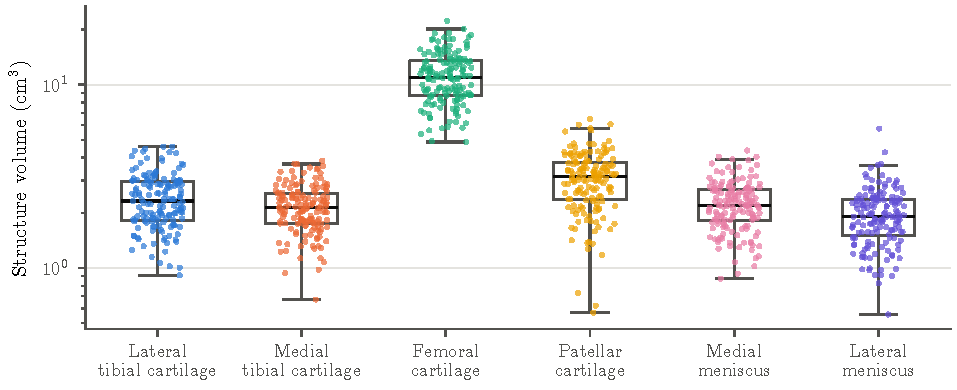
\includegraphics[width=\linewidth]{figures/ch4_structure_sizes.pdf}
\caption{Volume of each SKM-TEA structure over all 155 volumes (logarithmic axis). Boxes show the median and the interquartile range, whiskers extend to 1.5 times the interquartile range, and each point is one volume.}
\label{fig:ch4_structure_sizes}
\end{figure}

\begin{figure}[tb]
\centering
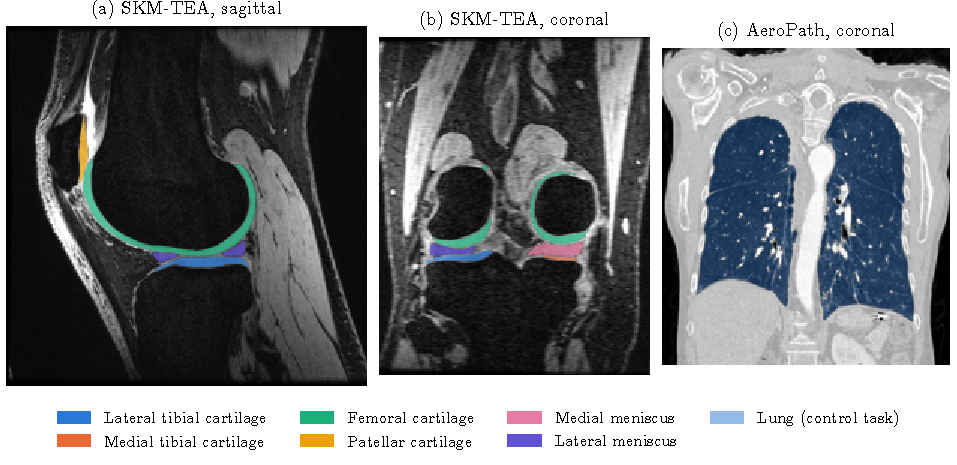
\includegraphics[width=\linewidth]{figures/ch4_examples.pdf}
\caption{Example volumes with their labels. (a)~Sagittal slice of SKM-TEA volume MTR\_005 through the lateral compartment, showing patellar, femoral and lateral tibial cartilage and the lateral meniscus. (b)~Coronal slice of the same volume through the tibial plateau, showing femoral cartilage, both tibial cartilages and both menisci. (c)~Coronal slice of AeroPath volume~1 with the lung label of the control task. Both example volumes belong to the test split.}
\label{fig:ch4_examples}
\end{figure}

% CLAUDE-DRAFT
We chose SKM-TEA because VoxTell performs poorly on it.
In the zero-shot evaluation of its authors, VoxTell reaches a mean Dice score of 10.72\,\% over the six SKM-TEA structures, with 46.45\,\% for femoral cartilage and at most 14.78\,\% for the other structures~\cite[Table~9]{rokuss2025voxtellfreetextpromptableuniversal}.
The authors attribute this to the knee being sparsely represented in the training data, and they name few-shot adaptation with minimal labelled examples as future work~\cite[p.~8]{rokuss2025voxtellfreetextpromptableuniversal}.
The knee is not entirely absent from VoxTell's training data, however: its label vocabulary contains femoral, patellar, and medial and lateral tibial cartilage from two knee \gls{mri} datasets, but no meniscus~\cite[Tables~4, 5 and~10]{rokuss2025voxtellfreetextpromptableuniversal}.
According to this vocabulary, SKM-TEA therefore combines structures that VoxTell has rarely seen with structures it has never seen.

% ---------------------------------------------------------------------
\section{AeroPath}
\label{sec:data-aeropath}

% CLAUDE-DRAFT
AeroPath contains 27 contrast-enhanced chest \gls{ct} scans (\gls{cta}), acquired with a thorax lung protocol at St.\ Olavs hospital in Trondheim, Norway~\cite{støverud2023aeropathairwaysegmentationbenchmark}.
The 27 patients, nine of them women, were aged 52 to 84 years (median 70) and were all undergoing diagnostic tests for lung cancer, with pathologies including malignant tumours, sarcoidosis and emphysema~\cite{støverud2023aeropathairwaysegmentationbenchmark}.
Data collection was approved by the Norwegian regional ethics committee (REK Sør-Øst~A, reference 2010/3385a), and written informed consent was obtained from the patients~\cite{støverud2023aeropathairwaysegmentationbenchmark}.
The dataset is distributed under the Creative Commons Attribution 4.0 licence\footnote{Zenodo record \url{https://zenodo.org/records/10069289}, DOI 10.5281/zenodo.10069289, accessed 19 October 2026.}.

% CLAUDE-DRAFT
In the files used here, the volumes have 487 to 512 by 407 to 512 voxels in-plane and 241 to 843 slices, with an in-plane voxel size of 0.56 to 0.82\,mm and a slice spacing of 0.50 to 1.25\,mm.
These ranges are wider than those stated in the dataset publication~\cite{støverud2023aeropathairwaysegmentationbenchmark}; we report the values of the files.
Each volume comes with an airway label and a lung label.
The publication describes how the airway labels were created, by region growing or grow-cut, an airway segmentation network and manual refinement verified by a pulmonologist~\cite{støverud2023aeropathairwaysegmentationbenchmark}.
How the lung labels were created is documented neither in the publication nor in the dataset repository or the Zenodo record.
We use only the lung label, with the text prompt ``lung''.

% CLAUDE-DRAFT
AeroPath serves as the control task.
It is never trained on, except by the strategy with replay, whose replay memory includes AeroPath training volumes.\todo{ref: Method, replay}
It measures how much of the pretrained model's ability on a structure outside the task sequence is lost during continual adaptation.
We chose it because the pretrained model segments it well and because it is public.
AeroPath is not part of VoxTell's training data: its authors use it as a held-out test set for a known concept, on which VoxTell reaches a lung Dice score of 96.99\,\%~\cite[Table~7]{rokuss2025voxtellfreetextpromptableuniversal}.
The concept itself is well represented in VoxTell's training data, where ``lung'' is among the most frequent labels~\cite[Table~10]{rokuss2025voxtellfreetextpromptableuniversal}.
How the loss of this ability is quantified is defined in the Method chapter.\todo{ref: control-task drop}

% ---------------------------------------------------------------------
\section{Data Splits and Few-Shot Subsets}
\label{sec:data-splits}

% CLAUDE-DRAFT
We split each dataset once, at random, into 70\,\% training, 15\,\% validation and 15\,\% test volumes.
The volumes are shuffled with a fixed random seed (42), the first 70\,\% of the shuffled list form the training split and the next 15\,\% the validation split, and the remaining volumes form the test split.
This gives 108 training, 23 validation and 24 test volumes for SKM-TEA and 19, 4 and 4 volumes for AeroPath.
Because the six tasks share the same volumes, every task uses the same split, and every experiment in this thesis uses the same split.
Each SKM-TEA patient contributes exactly one scan, so no patient appears in more than one split.
The validation volumes are used to select the checkpoint of each task; all reported results are computed on the test volumes.\todo{ref: Method, checkpoint selection}

% CLAUDE-DRAFT
SKM-TEA also defines an official split of 86 training, 33 validation and 36 test scans, in which the test scans are those of the 36 patients who received additional arthroscopic surgery~\cite{desai2021skmtea}.
We do not use this split, for two reasons.
First, the aim of this thesis is to compare continual-learning strategies with each other, not to compare results with published SKM-TEA benchmarks, which is the purpose of the official split; the comparison only requires that all strategies use the same split.
Second, the official test set consists of a selected group of patients, so a model trained on the official training split is tested under a shift between training and test data.
A random split keeps training and test volumes from the same distribution, so that differences in adaptation and forgetting are not mixed with the effect of such a shift.
\cref{tab:ch4_splits} shows how the official splits are distributed over our splits: 7 of our 24 test volumes belong to the official test set.
The results of this thesis are therefore not comparable with results reported on the official SKM-TEA test set.

\begin{table}[tb]
\centering
\caption{Number of SKM-TEA volumes in each split of this thesis (rows) and of the official SKM-TEA split~\cite{desai2021skmtea} (columns).}
\label{tab:ch4_splits}
% Generated by scripts/plot_data.py from results/data_stats. Do not edit.
\small\setlength{\tabcolsep}{6pt}
\begin{tabular}{lrrrr}
\toprule
 & \multicolumn{3}{c}{Official SKM-TEA split} & \\
\cmidrule(lr){2-4}
This thesis & Train & Val. & Test$^{a}$ & Total \\
\midrule
Training & 63 & 22 & 23 & 108 \\
Validation & 10 & 7 & 6 & 23 \\
Test & 13 & 4 & 7 & 24 \\
\midrule
Total & 86 & 33 & 36 & 155 \\
\bottomrule
\end{tabular}
\par\smallskip{\footnotesize $^{a}$ Patients with additional arthroscopic surgery.\par}

\end{table}

% CLAUDE-DRAFT
For the few-shot experiments, the training split of each task is reduced to its first $k$ volumes, with $k \in \{5, 10, 20\}$ labelled training volumes per task, in the order of the shuffled list.
The subsets are therefore nested, the 5 volumes being part of the 10 and the 10 part of the 20, and the same volumes are used for all six tasks.
For each $k$, one subset is drawn, so the results do not show how they vary with the choice of training volumes.
The full-data setting uses all 108 training volumes, and the validation and test volumes are the same in all settings.

% CLAUDE-DRAFT
Of AeroPath, only the 4 test volumes are used for evaluation.
The 19 training volumes are used only by the replay strategy, and the 4 validation volumes are not used.

% ---------------------------------------------------------------------
\section{Preprocessing}
\label{sec:data-preprocessing}

% CLAUDE-DRAFT
We convert each SKM-TEA \gls{hdf5} file into two \gls{nifti} files, one for the first echo and one for the labels.
The segmentation is stored as six binary channels, one per tissue; we convert it into a single label map in which each labelled voxel takes the index of its channel plus one and unlabelled voxels take the value zero.
Following the channel order of the official documentation, the label values are 1 for patellar cartilage, 2 for femoral cartilage, 3 for medial tibial cartilage, 4 for lateral tibial cartilage, 5 for medial meniscus and 6 for lateral meniscus.
For each task, the binary target mask consists of the voxels with the task's label value.
The \gls{nifti} files are written with an identity affine, so they store neither the voxel size nor the orientation of the scan.
Images and labels come from the same voxel grid and therefore stay aligned, which we checked visually in ITK-SNAP.\todo{cite: ITK-SNAP}
The AeroPath volumes and labels are used in their original \gls{nifti} format.

% CLAUDE-DRAFT
When a volume is loaded, it is reoriented according to its affine, which leaves the SKM-TEA volumes unchanged, and cropped to the bounding box of its non-zero voxels.
Its intensities are then normalised to zero mean and unit standard deviation over the cropped volume, using the z-score normalisation of nnU-Net~\cite{isensee2018nnunetselfadaptingframeworkunetbased}.
The same normalisation is applied to the \gls{mri} and the \gls{ct} volumes.
The volumes are not resampled.
The SKM-TEA volumes are therefore processed on their voxel grid as if the voxels were 1\,mm cubes, while the AeroPath volumes keep their physical voxel size.
How patches are sampled during training and how predictions are assembled during evaluation is described in the Method chapter.\todo{ref: Method, patch sampling and sliding-window inference}

% ---------------------------------------------------------------------
\section{Data Quality and Limitations}
\label{sec:data-limitations}

% CLAUDE-DRAFT
Several properties of the data limit the conclusions of this thesis.
Because of the identity affine, the SKM-TEA volumes reach the model at a different scale than their physical size: a voxel of $0.3125 \times 0.3125 \times 0.8$\,mm is treated as a 1\,mm cube, which enlarges the in-plane extent by a factor of 3.2 and the slice direction by a factor of 1.25.
The AeroPath volumes, in contrast, keep their physical voxel size, so the two datasets are processed at different scales.
Whether either scale matches the data on which VoxTell was pretrained cannot be checked from its publication, which does not state the voxel size used for training~\cite{rokuss2025voxtellfreetextpromptableuniversal}.\todo{defense: SKM-TEA scale and missing resampling may contribute to the low performance of the pretrained model on SKM-TEA; check the official VoxTell preprocessing}
The identity affine also removes the orientation: 18 of the 155 SKM-TEA scans are stored with the left--right axis reversed relative to the other 137, and the model receives them without this information.

% CLAUDE-DRAFT
The model sees only the first \gls{qdess} echo, although the annotators used both echoes to separate neighbouring cartilage and meniscus voxels~\cite[App.~A.4]{desai2021skmtea}.
Each SKM-TEA scan was labelled by one annotator, so the data contain no information on the agreement between annotators.
For AeroPath, the origin of the lung labels is not documented, so it is unknown whether they are manual or automatic references.
The control task is evaluated on only four test volumes, which makes its results less certain than those of the SKM-TEA tasks with 24 test volumes.
The \gls{ct} volumes are normalised per volume like the \gls{mri} volumes; whether this matches the normalisation used to pretrain VoxTell is not stated in its publication.\todo{defense: check VoxTell's CT intensity normalisation}
Finally, every result depends on one random split of each dataset and on one subset per number of training volumes.
   % Chapter 4: Data Description
\cleardoublepage
\include{method}   % Chapter 5: Method
\cleardoublepage
\include{experiment_results}   % Chapter 6: Experiment & Results
\cleardoublepage
\include{discussion}   % Chapter 7: Discussion
\cleardoublepage
\include{summary}   % Chapter 8: Summary
\cleardoublepage

\appendix
\cleardoublepage

   % appendix A
\cleardoublepage
%\include{thesis10}   % appendix B
%\cleardoublepage
%\include{thesis11}   % appendix C
%\cleardoublepage

%% Do not change, auto-generated lists of figures, tables and literature %%
% Glossar
\printunsrtglossary[type=abbreviations]
\cleardoublepage

% List of figures
\addcontentsline{toc}{chapter}{\listfigurename}
\listoffigures
\cleardoublepage

% List of tables
\addcontentsline{toc}{chapter}{\listtablename}
\listoftables
\cleardoublepage

% Literature list
% %CONFIG:
%\selectlanguage{german}{\addcontentsline{toc}{chapter}{\bibname}}
\selectlanguage{english}{\addcontentsline{toc}{chapter}{\bibname}}

\printbibliography
\end{document}
